\documentclass[11pt,letterpaper]{article}
\usepackage{array}
\usepackage[in]{fullpage}
\usepackage{verbatim}
\usepackage{parskip}
\usepackage{graphicx}
\usepackage{url}

\usepackage{titlesec}
\titlespacing{\section}{0pt}{\baselineskip}{0pt}
\titleformat*{\section}{\normalsize\bfseries\MakeUppercase}

\titlespacing{\subsection}{0pt}{0.5\baselineskip}{0pt}
\titleformat*{\subsection}{\normalsize\bfseries}

%\setlength{\parindent}{0in}

% precede modeling with a short discussion of motivation behind modeling
% 1. understanding vs. prediction
% 2. complex is not necessarily better. elegant is best!

\begin{document}
\textbf{ENVS S422: Earth's Climate System\\
Modeling Exercise 1: Introduction to systems modeling}\\

This modeling exercise is designed to give you familiarity with systems modeling in STELLA. The handout consists of (i) background on modeling, which you should use as a reference for future modeling exercises, and (ii) a series of simple model experiments that you will build and explore to gain an understanding of some important systems concepts. For each model experiment, you should submit a graph (with the exception of Section \ref{sec:residence_time}) and a brief 1-paragraph response to the questions that are being explored in the exercise. Each exercise in Section 3 is worth 5 points.

Due date: 9 September 2024

\section{Accessing STELLA}
STELLA is available on the university's virtual build, which you can access from your computer by follow the instructions here: \url{https://uas.alaska.edu/helpdesk/computers/central/virtual.html}. Once you've logged into the virtual machine, search for STELLA by typing ``stella 10.0''. 

\section{Background}
In order to illustrate some fundamental aspects of modeling and the behavior of dynamic systems, we'll start with the simplest system imaginable --- a tub of water with a faucet and drain.

\subsection{First steps} 
The first step in modeling is to define and consider the system as it actually exists in the real world. This involves identifying the components of the system, what material or entity is moving through the system, what processes are involved in moving this material or entity, and what kinds of things these processes are likely to depend on. This step is often facilitated by drawing a cartoon of the system, as shown in the schematic of the water tub (Figure \ref{fig:schematic}). 
\begin{figure}[h]
\begin{center}
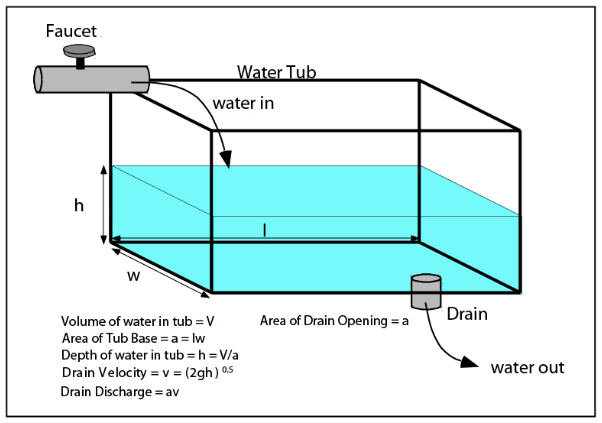
\includegraphics[]{./schematic.pdf}
\caption{A simple sketch of the water tub system, consisting of a faucet, a drain, and tub that contains water. The faucet flow rate is independently controlled, but the rate of flow through the drain is a function of the water depth and the area of the drain opening.}
\label{fig:schematic}
\end{center}
\end{figure}
The purpose of a schematic is to clarify what we are modeling, the components of the system, and the relationships between these components. No model can, nor should be expected to, perfectly replicate the real world. When developing a model, you have to make decisions about what physics to include, what to simplify, and what to discard. Some models are designed to try to elucidate the basic physics that influence a specific process, while other models attempt to make predictions about the future behavior of systems. The ultimate goal of a modeling effort determines the scope of the model and the amount of simplification that is acceptable or desired. If a model doesn't produce behavior that is consistent with observations, then the schematic should be revisited to assess whether important physics is missing from the model.

\begin{figure}[b!]
\begin{center}
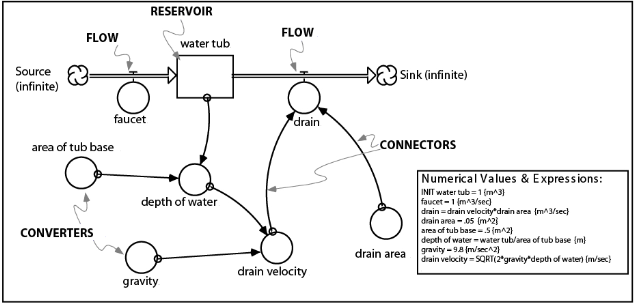
\includegraphics[]{./stella.pdf}
\caption{STELLA diagram of the faucet-tub-drain system that indicates the values and expressions of the reservoir, flows, and converters.}
\label{fig:tub}
\end{center}
\end{figure}

In the model that we will be exploring, the faucet can be adjusted to supply water at whatever flow rate we choose. In contrast, the rate of flow through the drain is going to be a function of the size of the drain opening and how much water is in the tub because the weight of the water overlying the drain determines the amount of pressure that is forcing the water through the drain. So, the outflow is dependent on the amount of water in the tub. A more precise description of this dependence is provided by Torricelli's Law, which states that the velocity of water flowing out of a drain is equal to the square root of two times the gravitational acceleration times the depth of the water above the drain. The velocity is multiplied by the area of the drain opening to give an outflow in volume of water per unit time.

Figure \ref{fig:tub} shows how this system is represented in STELLA using the four building blocks of systems: reservoirs, flows, connectors, and converters. A \textit{reservoir} is an amount of material (in this case the volume of water in the tub) and \textit{flows} represent movement of that material from one place to another. \textit{Connector arrows} indicate dependence; for example, the depth of water is dependent on the amount of water in the tub and the area of the tub base, so connector arrows go from the water tub reservoir and the tub area converter. \textit{Converters} are either constants or variables defined by equations or graphs. Note that the two flows have cloud symbols at the ends away from the tubes, indicating that this is an open system that draws water from an unspecified source and releases it to an unspecified sink.
 
\subsection{A word on units}
A very important step in setting up a model is to make sure that your units agree. Otherwise you won't really know what is being calculated when the model is being run. For this simple model of a water tub, we'll use units of meters and seconds. When you specify the model parameters in STELLA, you can also select the units for each reservoir, flow, and converter.

\subsection{Mathematics and numerical algorithms}
In mathematical terms, the flows in the STELLA models essentially represent rates of change. Thus, the models that you will be using throughout the semester consist of coupled differential equations. For some simple systems you may be able to find an \textit{analytical solution} (i.e., one that you derive by hand). As systems become more complex, analytical solutions become increasingly difficult/impossible to find. Computer methods for solving equations (and doing so efficiently) is an active area of research in scientific computing and numerical analysis. For our purposes, you should just know that STELLA uses a variety of finite difference schemes to integrate the model equations. In particular, you can choose between Euler's Method, Runge-Kutta 2, and Runge-Kutta 4. Due to the way that these algorithms work, you can get large numerical errors if you choose a time step that is ``too large''. One way to check whether your time step is too large is to run multiple simulations with different time steps and compare the results. A model that has time steps that are too large will likely produce erratic, nonphysical results. With the Runge-Kutta methods, computations take longer but you can get away with larger time steps.


\section{Systems concepts}
A number of important concepts connected to dynamic systems can easily be illustrated with a simple model of a water tub. Begin by building the model presented in Figure \ref{fig:tub}.

\subsection{Steady state\label{sec:steady_state}}
If you run the model for 100 s, you should observe the system evolving to a \textit{steady-state}, which means that the amount of water in the tub remains constant. Generate and submit a single plot that shows the temporal evolution of the inflow from the faucet, the outflow from the drain, and the volume of water in the tub. Include with the plot a brief description of the relationship between these model outputs.

\subsection{Residence time\label{sec:residence_time}}
Once the system is at (or at least very near to) steady state, we can calculate the \textit{residence time}. The residence time is the average length of time that an entity, in this case a water molecule, remains in a reservoir. By definition, the residence time is the amount of material in the reservoir, divided by either the inflow or the outflow (they are equal when the reservoir is in steady-state). If there are multiple inflows or outflows, then we use the sum of the inflows or outflows to determine the residence time. 

What is the residence time for the model run that you did in Section \ref{sec:steady_state}? Does the residence time for this simple system depend on the inflow? (To answer this, double the inflow and the model duration and run the model a second time.)

Residence time is an important concept in problems of pollutants in ground water or surface water reservoirs, and also in understanding the long-term effects of greenhouse gases added to the atmosphere.

\subsection{Response time}
DISCUSS E-FOLDING TIME!!!

A concept that is closely related to the residence time is the \textit{response time} of a system, which measures how quickly a system recovers and returns to its steady state after some perturbation. This concept can be illustrated by running several simulations in which you vary the initial state of the reservoir and observing how long it takes the system to reach a steady state. 

Set the model inflow back to 1~m$^3$/s and the model duration to 100~s. Run five simulations in which you vary the initial volume of the tub from 0--20~m$^3$ in increments of 5~m$^3$.

Submit a graph showing how the volume of water in the tub varies with time for each of the five simulations. To include all of the model results in one plot, you will need to set-up the graph before running any of the model simulations. Change the graph properties by setting the range of the graph from 0--20~m$^3$ and clicking the box labelled ``Comparative''; the latter holds the results from previous simulations. How does a perturbation to a volume of water in the tub affect the system's response time?

The concept of response time is important in many processes in Earth science, such as the evolution of the global carbon cycle. If we halt the anthropogenic emissions of CO$_2$, the response time of the system tells us how long it would take for the carbon cycle to return to a more natural state.

In this example, you should have always observed the system returning to the same steady state, which indicates that the steady-state of the system is primarily determined by the nature of the inflows and outflows. Later in the semester, we will explore systems that have multiple steady states.

\subsection{Feedback mechanisms}
This particular system returns to a steady state because it contains a \textit{negative feedback mechanism} in the connection between the drain flow rate and the amount of water in the tub. A negative feedback mechanism is a controlling mechanism that tends to counteract some kind of initial imbalance or perturbation. Note that the word negative, as used here, does not mean that it is bad feedback; it just means that the feedback mechanism acts to reverse the change that set the feedback mechanism into operation. So if our tub is in its steady state, knocking the system out of its steady state by suddenly dumping in more water will cause a response --- the drain will increase its flow rate, thus decreasing the volume of water in the tub and bringing it back towards the steady state value. If we instead decrease the amount in the tub, the negative feedback associated with the drain forces the amount of water in the tub to increase until the steady state is returned. The important thing to remember is that negative feedback mechanisms tend to have stabilizing effects on systems.

In contrast, a \textit{positive feedback mechanism} is one that exacerbates some initial change from the steady state, leading to a runaway condition --- it acts to promote an enhancement of the initial change. A simple way to modify the tub system in order to create a positive feedback system is to alter the inflow and outflow. This time, set the outflow to 1~m$^3$/s and let the inflow equal 0.2 times the volume of water in the tub. (To do this, you will need to delete most of the converters and connectors in the model.) For this experiment, run the simulation for 50 s.

Does this model have a steady-state? If so, what is the volume of water in the tub when it is in steady state? What happens if you increase or decrease the initial volume of water? Submit a comparative plot that illustrates how the water volume evolves for different initial volumes.

Positive feedback mechanisms, like negative feedback mechanisms, are not necessarily good or bad. Epidemics and infections have positive feedback mechanisms associated with them, but so does the growth of money in a bank account with compounded interest. The Earth contains a wide variety of both positive feedbacks and negative feedbacks. Depending on the conditions, either kind may dominate. The fact that we exist, and that our planet has water and an atmosphere, is compelling evidence to suggest that the Earth system is dominated by negative feedbacks mechanisms over long time scales. However, over time periods that matter to humans, positive feedback mechanisms may be very important and have the potential to produce dramatic changes.

\subsection{Lag time}
You will now build a slightly more complex system to investigate the concept of \textit{lag time}. In this model, two tubs are connected such that the water from the first tub drains into the second tub, which then drains out of the system. Set the initial volume of the tubs to 10~m$^3$ and the outflow from both tubs to 0.1 times the water volume. The inflow will vary with time, which you can describe in STELLA using a ``graphical function''. Set the inflow equal to ``TIME'', and then click the graph button below the equation definition. Modify the graph so that the inflow starts with a value of 1~m$^3$/s, then rapidly increases to a peak of 4~m$^3$/s and returns back to 1~m$^3$/s. Generate and submit a plot illustrating the variation in inflow and the water volume of both tubs. Describe the behavior that you observe and compare it to what you might expect for a flood propagating down a river.

The concept of a lag time is also relevant to systems such as the global carbon cycle. If we halt CO$_2$ emissions today, the climate will continue to warm.



%\section{Brief background}
%Daisyworld is a simple toy model that was developed to show that feedbacks within the Earth system can have a stabilizing effect on Earth's climate. The planet consists of uncovered land, white daisies, and black daisies. The area covered by daisies can grow or shrink as Earth's temperature fluctuates. The temperature depends on the solar radiation and the albedo of the uncovered land and daisies. That's basically it. Daisyworld doesn't contain an atmosphere, oceans, ice sheets, or mountains.
%
%\section{Daisyworld equations}
%\subsection{Planetary temperature}
%We will model Daisyworld by assuming that changes in the energy budget are slow. Thus we can assume that the rate at which energy is emitted by the planet equals the rate at which is energy absorbed by the planet. (Recall from the IPCC report that the at present the Earth is currently gaining energy, and so there is an energy imbalance. However, the current energy imbalance is just a small percent of the energy being received by the Earth.) The rate at which energy is emitted is given by the Stefan-Boltzmann Law:
%\begin{equation}
%\left(\frac{dE}{dt}\right)_{out}=\sigma\epsilon AT^4,
%\label{eq:stefan-boltzmann}
%\end{equation}
%where $\sigma=5.6704\times{10}^{-8}\mbox{ W/(m}^2\cdot\mbox{K}^4\mbox{)}$ is the Stefan-Boltzmann constant, $\epsilon$ is the emissivity, $A$ is the planet's surface area, and $T$ is temperature in kelvins. The emissivity is a dimensionless number between 0 and 1 that indicates how easily an object can emit energy. For simplicity, we will assume that $\epsilon=1$, so that Equation (\ref{eq:stefan-boltzmann}) becomes
%\begin{equation}
%\left(\frac{dE}{dt}\right)_{out}=\sigma AT^4,
%\label{eq:stefan-boltzmann2}
%\end{equation}
%
%The rate at which energy is absorbed by the planet equals the rate at which energy is received from the sun minus the rate at which energy is reflected back into space
%\begin{equation}
%\left(\frac{dE}{dt}\right)_{in}=IA-\left(\frac{dE}{dt}\right)_{ref},
%\label{eq:absorbed1}
%\end{equation}
%\noindent where $I$ is the irradiance, or rate at which energy is received from the sun per unit area. The rate at which energy is reflected is determined by the planetary albedo, $\alpha$, so that
%\begin{equation}
%\left(\frac{dE}{dt}\right)_{ref}=\alpha{IA}.
%\label{eq:reflected}
%\end{equation} 
%\noindent Albedo is a reflection coefficient between 0 and 1; when $\alpha=0$, none of the incoming radiation is reflected, and when $\alpha=1$, all of the incoming radiation is reflected. Combining Equations (\ref{eq:absorbed1}) and (\ref{eq:reflected}), we find that
%\begin{equation}
%\left(\frac{dE}{dt}\right)_{in}=IA(1-\alpha).
%\label{eq:absorbed2}
%\end{equation}
%Now, because we have assumed that the rates at which energy enters and leaves the planet are the same, we can equate Equations (\ref{eq:stefan-boltzmann2}) and (\ref{eq:absorbed2}) and divide by the surface area to find that
%\begin{equation}
%\sigma{T^4}=I(1-\alpha).
%\end{equation}
%Finally, rearranging gives
%\begin{equation}
%T=\left(\frac{I(1-\alpha)}{\sigma}\right)^{1/4}.
%\end{equation}
%Ultimately, this is the equation that we want to solve: How does Daisyworld's temperature vary with time? It depends on the irradiance, or incoming radiation from the sun, and the planetary albedo. The irradiance will be prescribed, while the albedo will depend on the growth of daisies, which depends on temperature. 
%
%
%\subsection{Solar irradiance}
%Daisyworld's sun begins with a diminished brightness (like all suns) and grows brighter with time. At the beginning of Daisyworld, it provides an irradiance of 550 $\mbox{W/m}^2$ to Daisyworld; two billion years later it is provides 1650 $\mbox{W/m}^2$. (The Earth currently receives 1366 $\mbox{W/m}^2$.) We will prescribe this change in irradiance with a simple linear equation:
%\begin{equation}
%I=550+\frac{1100t}{200},
%\end{equation}
%\noindent where $t$ is time in 10 million years (i.e., each time step equals 10 million years).
%
%\subsection{Planetary albedo}
%The albedo of Daisyworld is a function of how much area is covered by white daisies and black daisies. Uncovered land has an albedo of 0.5, while white daisies and black daisies have albedos of 0.75 and 0.25, respectively. The net planetary albedo, $A$, is
%\begin{equation}
%\alpha=A_{u}\alpha_{u}+A_w\alpha_w+A_b\alpha_b,
%\end{equation}
%\noindent where $a_{u}$, $A_w$, and $A_b$ are the fraction of the total area that is uncovered, covered with white daisies, and covered with black daisies (so that $A_{u}+A_w+A_b=1$), and $\alpha_{u}$, $\alpha_w$, and $\alpha_b$ are the albedos of the uncovered land, white daisies, and black daisies.
%
%The tricky part of this exercise is that the fractional areas will change with time, and the rate at which they change will depend on temperature. In particular, we will assume that the rate of fractional area change (for white daisies) is given by
%\begin{equation}
%\frac{d}{dt}A_w=A_w(g_w-d_w),
%\end{equation} 
%where $g_w$ and $d_w$ are the growth rate and death rate. This equation tells us that (1) if the growth rate exceeds the death rate, then the fractional area will increase, and (2) the rate of change depends on the area already covered by daisies. In other words, large amounts of daisies can die or be produced when the population is large. We will use an identical equation for black daisies.
%
%For the death rate, we will simply use a constant value of 0.3. This is equivalent to saying that, given a growth rate of 0, the fractional area of each type of daisy will decrease by 26\% during each interval of time (10 million years).
%
%The growth rate will depend on the local temperature near the daisies and the area of uncovered land, such that
%\begin{equation}
%g_w=A_u(1-0.003265(273+22.5-T_w)^2),
%\label{eq:growthrate}
%\end{equation}
%\noindent where $T_w$ is the local temperature in the vicinity of the white daisies. This equation looks complicated, but in reality it is just a parabola. The growth rate equals 0 when the temperature is 5$^\circ$C (278 K) and 40$^\circ$C (313 K), and reaches a maximum when the temperature is 22.5$^\circ$C (295.5 K). Furthermore, the growth rate depends on the area of uncovered land. If there is a lot of bare land, the daisies can spread more rapidly. One problem with Equation (\ref{eq:growthrate}) is that it gives negative growth rates for temperatures less than 5$^\circ$C or greater than 40$^\circ$C. We will need to account for this by using a ``conditional'' statement in our model.
%
%Finally, we want to account for the fact that the temperature near the white daisies will differ from the average global temperature. This can be calculate by
%\begin{equation}
%T_w=H_a(\alpha-\alpha_w)+T,
%\end{equation}
%\noindent where $H_a$ is a heat absorption factor. We will set $H_a=20$, which means that the temperature near the daisies will be 5$^\circ$C cooler than the average temperature on the planet (if $\alpha=0.5$ and $\alpha_w=0.75$).
%
%These equations describing daisy growth and death are a bit arbitrary and only loosely based on studies of population biology. In other words, don't take them too seriously. However, we can easily play with the equations to see how changing the conditions under which daisies thrive affects the stability of Daisyworld. The point here isn't to get an accurate portrayal of reality --- and in fact, we've already neglected the atmosphere, the oceans, and nutrient cycling --- instead, we're just trying to get an idea of how systems work and how non-intuitive they can be.
%
%\section{Implementation of Daisyworld}
%You will implement Daisyworld using the STELLA software package, which was specifically designed for systems modeling. It uses a fairly intuitive graphical interface. Your model should look similar to the one shown in the figure below.
%
%\begin{figure}[h]
%\includegraphics[width=4in]{./Daisyworld_model}
%\end{figure}
%
%Essentially, you will create the following items:
%\begin{enumerate}
%\item Reservoirs: Fractional areas of uncovered land, land covered by white daisies, and land covered by black daisies.
%\item Biflows: Arrows that indicate flow of ``stuff'' from one reservoir to another. In this exercise, if the area covered by daisies increases, there is a corresponding decrease in the uncovered area. You will need to set the initial uncovered area to 1, and the initial white daisy and black daisy areas equal to 0. Note that the black arrow in the biflow indicates the direction of flow if the rate of area change is negative.
%\item Converters: Use these to define equations or constants.
%\item Action connectors: These allow you to link various parameters within the model.
%\end{enumerate}
%
%\subsection{Experiments}
%\textbf{1. The standard case}
%
%You will begin with the model set-up as described above. However, before running the model, try to predict what will happen. What happens at first? Will both daisies start growing immediately? At the same time? Which type of daisies will live the longest? What is the combined effect of daisy growth on the planetary temperature?
%
%Now, run the model for 200 time units, using a time step of 0.25 time units. It will be instructive to plot the three reservoirs on one graph, and the average planetary temperature and the temperature of a ``dead'' planet on another graph. Other graphs may be necessary to fully understand what is driving the observed behavior.\\
%
%\textbf{2. Changing albedos}
%
%Initially, the black albedo is set at 0.25, while the white albedo is 0.75. In this experiment, modify these albedos, first to more
%extreme values (.05 and .95) and then to more moderate values (.4 and .6). Be sure to make some careful predictions before running
%these models.\\
%
%\textbf{3. Changing growth factor curve}
%
%One of the critical parts of this model is the growth factor for daisy growth. In this experiment, we will alter the growth factor and
%see how the model responds.
%
%a) First, alter the optimum temperature for the daisies' growth, which is initially set at 22.5$^\circ$C, to 15$^\circ$C. To do this, alter the equations for the growth factors, replacing 22.5 with 15. As always, make predictions before running the model.
%
%b) Next, restore the optimum temperature to 22.5$^\circ$C and then reduce the range of temperatures that the daisies can tolerate. Initially,
%the daisies can grow in temperatures ranging from 5 to 40. Now restrict the range so that the daisies grow only between 18 and 27;
%this can be done by replacing the 0.003265 with 0.05 in the equations for the growth factors. You will also need to adjust the conditional statement to ensure that the growth rate isn't negative outside of this temperature range. As always, make predictions before running the model.\\
%
%\textbf{4. Plagues}
%
%This experiment explores the resilience of Daisyworld by programming a set of plagues into the model. These plagues decimate the
%populations periodically for brief periods. An interesting question here is whether or not the daisies will be able to recover fast
%enough to return the planetary temperature to the "comfort zone". To implement this change, double-click on the death rate
%converter and replace 0.3 with "time" (without the quotation marks), then click on the Graph button in the lower left of the
%window, and check the ``graphical'' radio button. Next set the number of data points to 101; this should give you one input value every 2 time units, thus allowing us to make fairly brief plagues (still, these are 20 Myr long!). Then, set the scale on the graph to 0.3, and click and drag the graph until all of the time steps have a death rate of 0.3. Next, click on the points tab, and manually change the death rate to a value of 1.0 at time
%units 50, 100, and 150 (and others, if you'd like); click on the OK button and the plagues should be inserted into the model. Run the model as before, after making a prediction about what will happen. Are all of the plagues equal in magnitude (in terms of area lost as a result of the
%deaths)? Does each plague result in the same kind and magnitude of temperature change? Does the system recover from each
%plague? What determines whether or not the planet recovers from a plague?\\
%
%\textbf{5. Volcanic eruptions}
%
%Now investigate how Daisyworld responds to volcanic eruptions, which put ash into the air and reduce the amount of energy that enters the planet (assume that the ash doesn't affect the outgoing radiation). To do this, use a conditional statement for the irradiance equation to reduce the incoming radiation during a short time interval (e.g., one time step). How long does it take Daisyworld to recover? Try using different time intervals. Can you extend or shorten the life of one of the daisies?

\end{document}
